\documentclass[a4paper, 11pt]{article}

\usepackage[spanish]{babel} % Idioma
\usepackage[utf8]{inputenc} % Codificación
\usepackage[T1]{fontenc} % Codificación
\usepackage{adjustbox} % Tamaño de tablas
\usepackage{float} % Posicionamiento de figure
\usepackage[vmargin=2cm,hmargin=2cm]{geometry} % Márgenes
\usepackage{graphicx} % Imágenes
\usepackage{hyperref} % Enlaces
\graphicspath{{img/}} % Las imágenes están en la carpeta img
\usepackage{accents} % Cosas de Windows
\usepackage{framed} % Frames

\newcommand{\spec}[6]{
\bgroup
\def\arraystretch{1.2}
\begin{tabular}{|l|}
\hline
Ejecución en el PC de \textbf{#1} con optimización -O#6:\\
CPU: #2 @#3 GHz\\RAM: #4 GB \hspace{0.8cm} SO: #5 \\
\hline
\end{tabular}
\egroup
\vspace*{0.2cm}
}

\title{\Huge \textbf{Práctica 2}}

\author{\textbf{Pablo Baeyens Fernández} \\ \textbf{Antonio Checa Molina} \\
\textbf{Iñaki Madinabeitia Cabrera} \\  \textbf{José Manuel Muñoz Fuentes} \\
\textbf{Darío Sierra Martínez} \\ }
\date{Algorítmica}



\begin{document}

\maketitle
\tableofcontents
\section{El elemento en su posición}

La implementación de todos los algoritmos realizados es de la forma:
\begin{description}
 \item[Entrada:] Vector ordenado \texttt{v} (sin repetidos) y su tamaño \texttt{n}
 \item[Salida:] Entero no negativo que indica el $i$ tal que $v[i]=i$ en caso de que exista o $-1$ en otro caso
\end{description}

Es decir, estos algoritmos deberan encontrar un elemento en su posición o deducir que no existe tal elemento. En el caso del algoritmo recursivo necesitamos un parámetro adicional para pasar información adicional, pero utilizamos una función \textit{wrapper} que incializa este parámetro adecuadamente.

\subsection{Descripción de los algoritmos y eficiencia teórica}

El algoritmo \textbf{obvio} que resuelve el problema de \textit{El elemento en su posición} consiste
en recorrer cada elemento del vector y comprobar para cada uno de estos si se cumple la
condición deseada ($v[i] = i$):

% Versión obvia
\lstinputlisting[firstline=23, lastline=28]{cpps/posicion.cpp}

Las condiciones de comienzo, actualización y final del bucle son todas $O(1)$, así como el código del interior del bucle. El bucle se ejecutará un máximo de \texttt{n} veces, por lo que es claro que la eficiencia de este algoritmo es de $\mathbf{O(n)}$.

\vspace*{1cm}
\hrulefill
\vspace*{1cm}

Para el algoritmo \textbf{divide y vencerás} hemos realizado dos versiones. La primera de ellas realiza el algoritmo de forma recursiva mientras que la segunda de forma no recursiva. Dada la similitud de nuestro problema con la búsqueda en un vector, nos hemos inspirado en la búsqueda binaria para realizar el siguiente algoritmo:

% Versión recursiva
\lstinputlisting[firstline=60, lastline=72]{cpps/posicion.cpp}

El parámetro \texttt{ajuste} nos sirve para ajustar la comprobación de la posición en función de la posición en la que estemos en el vector.
El caso base utiliza el algoritmo obvio ajustado (la condición que se comprueba es en este caso $v[i]-ajuste == i$), y se utiliza para los vectores de tamaño $\leq 3$, (el umbral encontrado en la siguiente sección).

Si el tamaño del vector es mayor que 3, comprobamos (ajustando) el elemento en el medio.
Distinguimos 3 casos:

\begin{itemize}
  \item El elemento medio está en su posición. En este caso devolvemos este elemento.
  \item $m < v[m]$ (ajustando). En este caso nos basta comprobar el lado izquierdo del vector, ya que $\forall k > 0, v[m + k] \geq v[m] + k > m + k$.
  \item $m > v[m]$ (ajustando). En este caso basta comprobar el lado derecho por un argumento similar, ya que $\forall k > 0, v[m - k] \leq v[m] - k < m - k$.
\end{itemize}

En caso de que no encontremos el elemento en lado adecuado devolvemos $-1$, que nos indica que no existe ningún elemento en su posición.

La \textbf{eficiencia} teórica de este algoritmo puede calcularse a partir de su ecuación de recurrencia, de la forma:

\[
T(n) = \begin{cases} T(n/2) + O(1) & \mbox{si } n > 3 \\
O(1) & \mbox{si } n \leq 3 \end{cases}\]

Sustituyendo $n = 2^k$ obtenemos que el orden de eficiencia de este algoritmo es $\mathbf{O(\log(n))}$.

\vspace*{1cm}
\hrulefill
\vspace*{1cm}

La versión no recursiva:

% Versión no recursiva
\lstinputlisting[firstline=87, lastline=101]{cpps/posicion.cpp}


Es la misma idea que la del algoritmo recursivo, dividiendo el vector en trozos más pequeños, sólo que para hacerlo iterativamente necesitamos un bucle \texttt{while} y unos límites que controlen las dimensiones de los trozos con los que nos vamos quedando del vector, llamados \texttt{tope_min} y \texttt{tope_max}.  Si encontramos un número que coincida con su posición, devolvemos el número. Si no lo encontramos (muy necesaria la comprobación $\texttt{tope_max} \geq \texttt{tope_min}$), se devuelve -1.

Al ser la misma idea que el algoritmo recursivo, pero de forma iterativa, la \texbf{eficiencia} teórica es la misma. Es decir, es  $\mathbf{O(\log(n))}$.

\subsection{Determinación del umbral}

En el caso del algoritmo divide y vencerás hemos hecho un estudio del mismo para determinar el umbral para el caso base (para el cual utilizamos el algoritmo obvio) que resulta más eficiente.

%% TODO: (Antonio) Estudio del umbral

Hemos buscado el punto de corte entre ambos algoritmos, para ver cuándo el algoritmo obvio empieza a ser menos eficiente que el divide y vencerás. Para sacar los datos del lineal no hemos tenido problemas, pero sí surgieron errores cuando queríamos compararlo con el divide y vencerás, que tardaba demasiado poco, y cualquier mínimo error movía la gráfica lo suficiente para que no se pudiera determinar nada.

Para poder estabilizar los datos y poder compararlos tuvimos que realizar una media de medio millón de ejecuciones, y realizar la gráfica de esos datos. Los datos de las ejecuciones son los siguientes:

\vspace*{1cm}

\pgfplotstableread{dats/posicion_t_50.dat}\posObvioComp
\pgfplotstableread{dats/posicion_1_50.dat}\posDyVComp
%\pgfplotstableread{dats/comp_umbral_posicion/posicion_2.dat}\posDyVTwo
\pgfplotstablecreatecol[copy column from table={\posDyVComp}{[index] 1}] {par1} {\posObvioComp}
%\pgfplotstablecreatecol[copy column from table={\posDyVTwo}{[index] 1}] {par2} {\posObvio}

\pgfplotstabletypeset[
display columns/0/.style={column name=Tamaño},
display columns/1/.style={column name=Algoritmo Obvio},
display columns/2/.style={column name=Algoritmo DyV (rec)}
%display columns/3/.style={column name=Algoritmo DyV (no rec)},
]{\posObvioComp}

\vspace*{1cm}

Y las gráficas que muestran los datos:
\begin{figure}[H]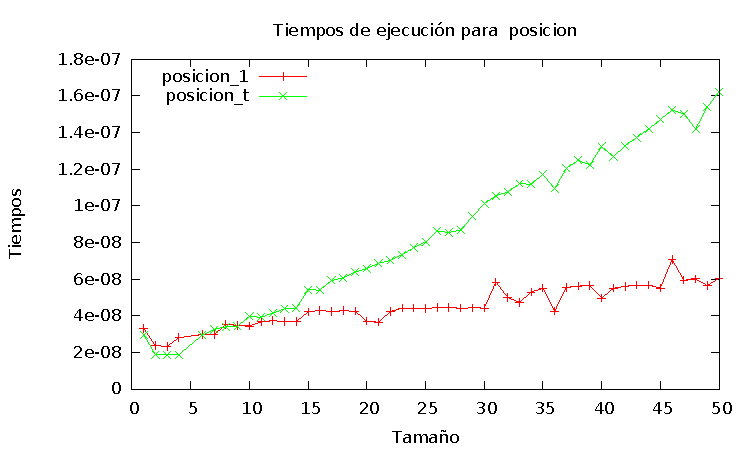
\includegraphics[width=13cm]{img/posicion_todos1_g_50.pdf} \centering
	\caption{Comparativa de tiempos en tamaños chicos para ver el umbral óptimo}\end{figure}

Vimos que el punto de corte estaba cerca del 6, aunque luego cuando estuvimos probando umbrales, el óptimo apareció en el 3, como se verá justo a continuación.

\subsection{Comparación de algoritmos}

A continuación mostramos las tablas y gráficas de comparaciones de diferentes umbrales, junto a sus funciones híbridas. Cogimos los umbrales cercanos al punto de corte anteriormente mencionado:

\vspace*{1cm}

\pgfplotstableread{dats/comp_umbral_posicion/posicion_t.dat}\posObvioCompUmbral
\pgfplotstableread{dats/comp_umbral_posicion/posicion_1.dat}\posDyVUmbralOne
\pgfplotstableread{dats/comp_umbral_posicion/posicion_1_umbral_2.dat}\posDyVUmbralTwo
\pgfplotstableread{dats/comp_umbral_posicion/posicion_1_umbral_3.dat}\posDyVUmbralThree
\pgfplotstableread{dats/comp_umbral_posicion/posicion_1_umbral_4.dat}\posDyVUmbralFour
\pgfplotstableread{dats/comp_umbral_posicion/posicion_1_umbral_5.dat}\posDyVUmbralFive
\pgfplotstablecreatecol[copy column from table={\posDyVUmbralOne}{[index] 1}] {par1} {\posObvioCompUmbral}
\pgfplotstablecreatecol[copy column from table={\posDyVUmbralTwo}{[index] 1}] {par2} {\posObvioCompUmbral}
\pgfplotstablecreatecol[copy column from table={\posDyVUmbralThree}{[index] 1}] {par3} {\posObvioCompUmbral}
\pgfplotstablecreatecol[copy column from table={\posDyVUmbralFour}{[index] 1}] {par4} {\posObvioCompUmbral}
\pgfplotstablecreatecol[copy column from table={\posDyVUmbralFive}{[index] 1}] {par5} {\posObvioCompUmbral}

\pgfplotstabletypeset[
display columns/0/.style={column name=Tamaño},
display columns/1/.style={column name=Algoritmo Obvio},
display columns/2/.style={column name=Umbral 1},
display columns/3/.style={column name=Umbral 2},
display columns/4/.style={column name=Umbral 3},
display columns/5/.style={column name=Umbral 4},
display columns/6/.style={column name=Umbral 5},
skip rows between index={25}{50}
]{\posObvioCompUmbral}

\vspace*{1cm}

Y las gráficas de los mismos:

\begin{figure}[H]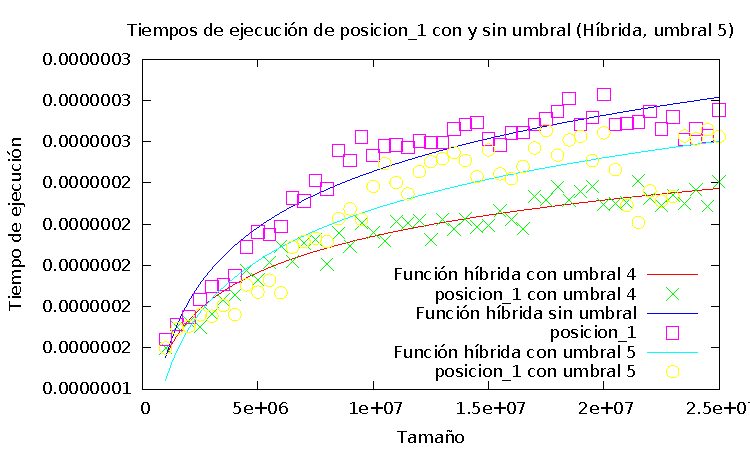
\includegraphics[width=13cm]{img/posicion_1_comparativa_umbral2.pdf} \centering
	\caption{Tiempos y funciones híbridas de umbrales 4 y 5}\end{figure}

Como poner los 5 umbrales y sus híbridas haría que la gráfica fuera un poco caótica, hemos decidido poner una gráfica solo con las híbridas de los algoritmos, para que se vea la tendencia de los tiempos, que es lo que importa:

\begin{figure}[H]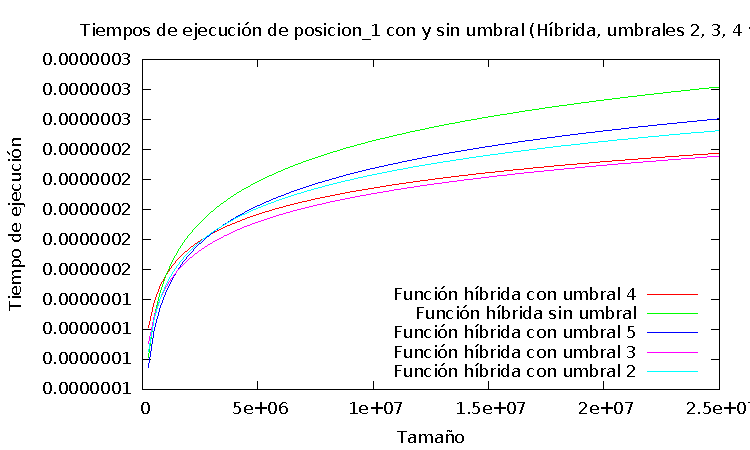
\includegraphics[width=13cm]{img/posicion_1_comparativa_umbral5.pdf} \centering
	\caption{Tiempos y funciones híbridas de umbrales 2, 3, 4 y 5}\end{figure}

En la gráfica ya podemos observar que el umbral 3 y 2 son prácticamente iguales, y los preferibles. La gráfica va aumentando conforme nos alejamos de estos dos números, como se puede ver que los umbrales 4 y 5 se encuentran un poco más arriba.

Hemos conseguido bajar un cuarto el tiempo de ejecución solo jugando con el umbral, así que remarcamos la importancia de encontrar el óptimo en un algoritmo Divide y Vencerás.

Por último colocamos una gráfica 3D de cómo varían los tiempos en función del umbral y del tamaño.

\begin{figure}[H]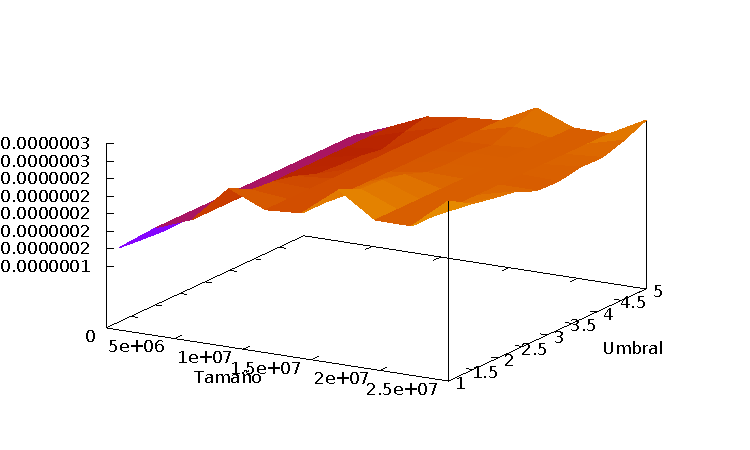
\includegraphics[width=13cm]{img/umbral_posicion.pdf} \centering
	\caption{Tiempos según Umbral y Tamaño}\end{figure}

\subsection{Eficiencia empírica de los algoritmos}

Utilizando la librería \texttt{chrono} hemos medido los tiempos de los algoritmos para un conjunto fijo de tamaños. Aunque los algoritmos son rápidos para tamaños grandes, las funciones auxiliares utilizadas para la generación de muestras aleatorias que permitan medir el tiempo han dificultado la obtención de los datos. Los datos obtenidos pueden verse en la siguiente tabla:


% tex.stackexchange.com/questions/10284

\vspace*{1cm}

\pgfplotstableread{dats/comp_umbral_posicion/posicion_t.dat}\posObvio
\pgfplotstableread{dats/comp_umbral_posicion/posicion_1.dat}\posDyV
%\pgfplotstableread{dats/comp_umbral_posicion/posicion_2.dat}\posDyVTwo
\pgfplotstablecreatecol[copy column from table={\posDyV}{[index] 1}] {par1} {\posObvio}
%\pgfplotstablecreatecol[copy column from table={\posDyVTwo}{[index] 1}] {par2} {\posObvio}

\pgfplotstabletypeset[
display columns/0/.style={column name=Tamaño},
display columns/1/.style={column name=Algoritmo Obvio},
display columns/2/.style={column name=Algoritmo DyV (rec)},
skip rows between index={25}{50}
%display columns/3/.style={column name=Algoritmo DyV (no rec)},
]{\posObvio}

\vspace*{1cm}

Podemos ajustar estos datos con una función representativa del orden de eficiencia teórico obtenido en la sección anterior:

%% TODO: (¿?) Ajustes de las funciones

En el siguiente gráfico podemos observar además una comparativa de las eficiencias empíricas y teóricas de los algoritmos realizados:



%% TODO: (Antonio) Gráfica con todos los algoritmos

\subsection{Vectores con elementos repetidos}

En el caso de que tengamos elementos repetidos el razonamiento realizado para justificar el algoritmo divide y vencerás no es válido, y es sencillo encontrar ejemplos de vectores con elementos en su posición para los cuales nuestro algoritmo no funciona.

Consideremos por ejemplo el caso del vector $v = [1,2,2]$. $1 <v[1]$, por lo que nuestro algoritmo comprobaría sólo el lado izquierdo ($[1]$) y no encontraría el elemento en la posición 2, que está en su posición.

Podemos plantear otro algoritmo de carácter similar para encontrar un elemento en su posición en estos casos:

\lstinputlisting[firstline=111, lastline=135]{cpps/posicion.cpp}

Este algoritmo realiza la búsqueda en el mismo orden en el que la haría el recursivo, solo que si no encuentra el número, hace también la otra mitad del vector. Este comportamiento provoca que se comporte casi logarítmico cuando hay un elemento en su posición, y peor que lineal cuando no se encuentra.

Por tanto, la eficiencia de este algoritmo depende drásticamente en la probabilidad de que un elemento esté en su posición y en la probabilidad de repetidos. Cuando más repetidos y menos en su posición, peor. Como en una distribución uniforme sobre el rango de elementos en los que trabajamos la probabilidad de que un elemento caiga en su posición es bastante baja, por mucho que a veces sea logarítmico, no compensa las veces que es peor que lineal.

Para comparar este algoritmo con los demás hemos necesitado de nuevo realizar una media de varios miles de ejecuciones para que se pudiera ver de forma decente lo que pasaba. A continuación dejamos las tablas y gráficos que lo muestran:

\section{Comparación de preferencias}

En esta sección se presentan algoritmos que cumplen:
\begin{description}
	\item[Entrada:] Vector de enteros \texttt{v} y su tamaño \texttt{n}
	\item[Salida:] Entero no negativo que indica el número de pares $i,j$ de posiciones del vector tales que $i < j$ y $v[i] > v[j]$
\end{description}

Es decir, estos algoritmos deberán contar el número de elementos que se encuentran invertidos en el vector.

\subsection{Algoritmo obvio}

El algoritmo que hemos considerado \textbf{obvio} para comprobar el número de inversiones es el siguiente, que simplemente comprueba todas las parejas posibles de elementos del vector y añade $1$ a un contador para cada pareja invertida, devolviendo el valor del contador al final de la ejecución. Esta es su implementación en C++:

\lstinputlisting[firstline=24, lastline=32]{cpps/preferencias.cpp}

El contenido del bucle interno se ejecuta:
\[\sum_{i=0}^{n-2} n-i+1 = \frac{n^2}{2}+\frac{3n}{2}-2\]
veces, por lo que, dado que la inicialización y actualización del bucle y las condiciones comprobadas se realizan en un tiempo constante, es un algoritmo de orden de eficiencia $O(n^2)$.

\subsection{Inversiones y algoritmos de ordenación: Divide y Vencerás}

No pudimos evitar darnos cuenta de la proximidad de nuestro problema con la ordenación de datos. Al ordenar datos, se deshacen las inversiones, y si hay un algoritmo de ordenación que facilite seguir la pista al proceso de deshacer inversiones, podemos aprovecharlo para contar el número de inversiones efectuado.
Por ello buscamos un algoritmo de ordenación con un orden de eficiencia mejor que el del algoritmo obvio (cuadrático) que se pareciese lo máximo posible a nuestro problema.

El primer candidato fue el \textit{quicksort} por su rapidez. Sin embargo, no es adecuado para ayudarnos con esta cuestión, pues presenta un comportamiento difícil de controlar en cuanto a inversiones, dado que puede añadir inversiones en el proceso.

A continuación analizamos el algoritmo \textit{heapsort} dado que nos pareció que las propiedades del \textit{heap}, un árbol parcialmente ordenado, podrían arrojar algo de luz al problema; aunque al final resultó que precisamente la estructura de árbol lo hacía un inadecuado candidato.

Por último llego el turno del \textit{mergesort}. Este algoritmo divide el vector original en subvectores, combinando las soluciones. Pero tiene una forma de hacerlo más simple que el resto: tanto en el caso base (en el que se usará inserción) como en la mezcla de vectores podemos controlar el número de inversiones deshechas.

Por debajo de un cierto umbral aplicamos el algoritmo de ordenación por inserción, un algoritmo que en cada uno de sus pasos deshace una inversión, por lo que puede usarse este mismo algoritmo para contar el número de inversiones con una variable que se incremente a cada inversión realizada. Resulta más rápido que el algoritmo trivial en este menester, pero sigue siendo $O(n^2)$, y, curiosamente, al usar optimización se invierten los papeles y el algoritmo trivial es más rápido que el algoritmo de inserción. \\

A la hora de mezclar vectores también puede controlarse el número de inversiones deshechas. Consideremos un vector $T$, lo partimos en dos y aplicamos inserción a cada una de sus partes: izquierda ($U$) y derecha ($V$). Se observa que, al ordenar cada parte, las inversiones de los elementos de una parte respecto de elementos de la otra se conservan. Por ello, si en la mezcla de dos vectores $U$ y $V$ se inserta un elemento de $V$ cuando quedan $k$ elementos de $U$ por insertar, se estarán deshaciendo $k$ inversiones. Entonces el número de inversiones de $T$ será el número de inversiones de $U$ más el número de inversiones de $V$ más la suma de cada $k$ obtenido en cada inserción de un elemento de $V$ en la mezcla.\\

Veamos un ejemplo:

\[[5,4,3,2,1]\]

El elemento $a_i$ de está lista está invertido $n-i$ veces con respecto a los demás. Apliquemos el $mergesort$:

\[[5,4,3] \hspace{1cm} [2,1]\]

Si lo ordenamos los elementos del vector izquierdo siguen estando invertidos con respecto a los del derecho:

\[[3,4,5] \hspace{1cm} [1,2]\]

Ahora unamos las soluciones. Tomamos un índice al principio de cada vector; empezamos añadiendo elementos de $U$ hasta que encontremos uno de $V$ menor. Si $j$ es el indice de $U$ por el que nos hemos parado y $n$ su tamaño, el elemento que vamos añadir de $V$ está invertido con respecto de $n-(j-1)$ elementos del vector $U$.

Por tanto el número de inserciones de un vector es igual al de $U$ más el de $V$ más el de los contados al unir las soluciones.

Mediante este razonamiento y una leve modificación del algoritmo \textit{mergesort} obtenemos una mejora sustancial al algoritmo trivial; una solución Divide y Vencerás de orden $O(n\cdot \log(n))$, que usa el algoritmo de inserción por debajo de cierto umbral.

\subsection{Determinación del umbral}

Se ha hallado el umbral óptimo en el siguiente contexto:

\spec{Darío}{\href{http://ark.intel.com/products/75116}{Intel\textregistered\ Core\texttrademark\ i7-4700HQ}}{2.40}{12}{Ubuntu 14.04 64 bits}{0}

Para hallar el umbral se han obtenido los tiempos de ejecución del algoritmo de inserción con conteo de número de inversiones (que se usará como caso básico para el Divide y Vencerás) y los tiempos de ejecución del algoritmo Divide y Vencerás basado en \textit{mergesort} con umbral 2 (es decir, aplicando Divide y Vencerás siempre excepto con subvectores de tamaño 2), con los siguientes tiempos en segundos:


\vspace*{1cm}

\pgfplotstableread{dats/preferencias_i.dat}\prefIns
\pgfplotstableread{dats/preferencias_d_sinumbral.dat}\prefDVt
\pgfplotstablecreatecol[copy column from table={\prefDVt}{[index] 1}] {par1} {\prefIns}

\pgfplotstabletypeset[
display columns/0/.style={column name=Tamaño},
display columns/1/.style={column name=Inserción},
display columns/2/.style={column name=Mergesort},
]{\prefIns}

\vspace*{1cm}

Que se representan con la siguiente gráfica:

\begin{figure}[H]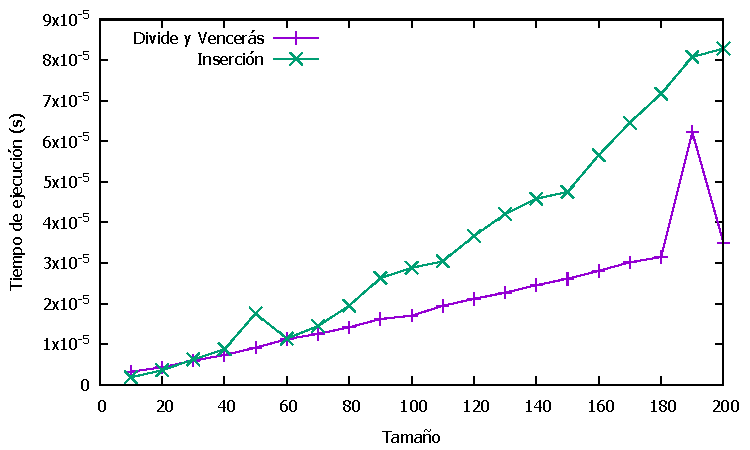
\includegraphics[width=14cm]{img/umbral_preferencias.pdf} \centering
	\caption{Tiempos según tamaño}
\end{figure}

El tiempo de ejecución del algoritmo basado en la ordenación por inserción se ajusta a la función $i(n) = 1.56413 \cdot 10^{-9} n^2 + 9.84525 \cdot 10^{-8} n + 2.08435 \cdot 10^{-6}$, mientras que el tiempo obtenido con el algoritmo derivado del \textit{mergesort} (ignorando el resultado obtenido en tamaño $190$) tiene por función de ajuste $m(n) = 3.08096 \cdot 10^{-8} n \cdot \log(n) + 3.07834 \cdot 10^{-6}$. Hallamos el punto de corte usando la función \texttt{find\_root} de Maxima:

\begin{lstlisting}[language=Maxima]
	i(n):=1.56413*10^(-9)*n^2 + 9.84525 * 10^(-8)*n + 2.08435*10^(-6)$
	m(n):=3.08096*10^(-8)*n*log(n) + 3.07834*10^(-6)$
	find_root(m(x)-i(x),x,10,200);
\end{lstlisting}

Obteniendo el punto de corte $25.726267$. Sin embargo, en pruebas posteriores de umbrales cercanos a ese punto de corte, hemos concluido que el umbral óptimo resultó estar alrededor de $50$.

\subsection{Comparación de algoritmos}

La tabla anterior recogía los tiempos obtenidos con el algoritmo basado en la ordenación por inserción y con el algoritmo basado en \textit{mergesort} con umbral $2$. En la siguiente tabla se completa con los tiempos obtenidos con el umbral considerado óptimo, $50$ (el número a continuación de \textit{Mergesort} es el umbral usado), y los tiempos con el algoritmo trivial:

\vspace*{1cm}

\pgfplotstableread{dats/preferencias_d.dat}\prefDVf
\pgfplotstableread{dats/preferencias_t.dat}\prefObv
\pgfplotstablecreatecol[copy column from table={\prefDVt}{[index] 1}] {par1} {\prefDVf}
\pgfplotstablecreatecol[copy column from table={\prefIns}{[index] 1}] {par2} {\prefDVf}
\pgfplotstablecreatecol[copy column from table={\prefObv}{[index] 1}] {par3} {\prefDVf}

\pgfplotstabletypeset[
display columns/0/.style={column name=Tamaño},
display columns/1/.style={column name=Mergesort $50$},
display columns/2/.style={column name=Mergesort $2$},
display columns/3/.style={column name=Inserción},
display columns/4/.style={column name=Algoritmo obvio},
]{\prefDVf}

\vspace*{1cm}

Que se ilustran con esta gráfica:

\begin{figure}[H]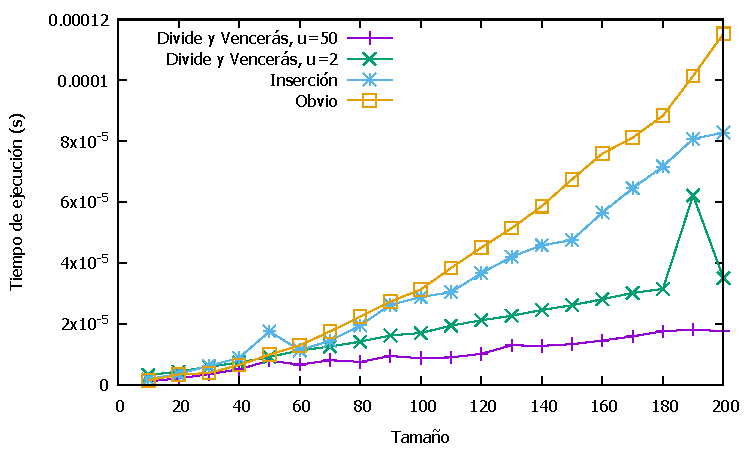
\includegraphics[width=14cm]{img/comparativa_preferencias.pdf} \centering
	\caption{Tiempos según tamaño para cada algoritmo}
\end{figure}

Además hemos repetido las ejecuciones con valores mayores para el algoritmo Divide y Vencerás con los dos umbrales, obteniendo esta tabla:

\vspace*{1cm}

\pgfplotstableread{dats/comp_umbral/preferencias_d_umbral.dat}\prefDVu
\pgfplotstableread{dats/comp_umbral/preferencias_d_sinumbral.dat}\prefDVs
\pgfplotstablecreatecol[copy column from table={\prefDVs}{[index] 1}] {par1} {\prefDVu}

\pgfplotstabletypeset[
display columns/0/.style={column name=Tamaño},
display columns/1/.style={column name=Mergesort $50$},
display columns/2/.style={column name=Mergesort $2$},
skip rows between index={25}{50}
]{\prefDVu}
\pgfplotstabletypeset[
display columns/0/.style={column name=Tamaño},
display columns/1/.style={column name=Mergesort $50$},
display columns/2/.style={column name=Mergesort $2$},
skip rows between index={0}{25}
]{\prefDVu}

\vspace*{1cm}

Y la gráfica siguiente:

\begin{figure}[H]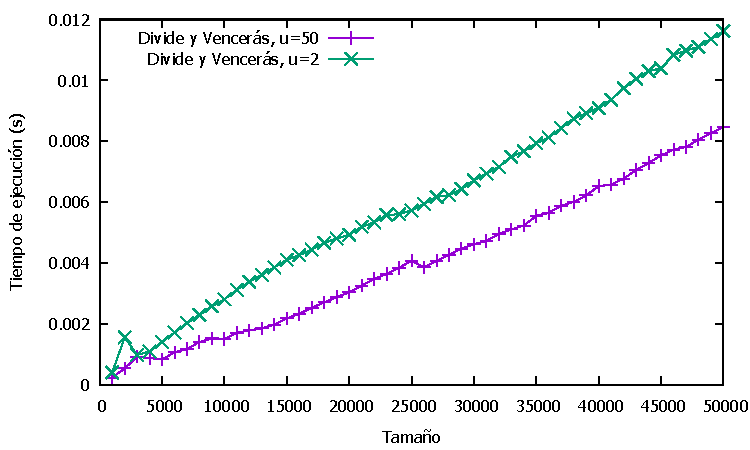
\includegraphics[width=14cm]{img/comparativa_preferencias_grande.pdf} \centering
	\caption{Tiempos según tamaño para Divide y Vencerás}
\end{figure}

Cabe destacar que los tiempos de ejecución del algoritmo trivial para valores en torno a $50\ 000$ se encuentran aproximadamente tres órdenes de magnitud por encima de los obtenidos para el algoritmo Divide y Vencerás con el umbral $50$.

\end{document}
